\scanpage{68}
\mspage{67}
\mspage{29}
\[
(u^*(R^1j_*)g^*F)_{\overline x}\simeq((R^1j_*)g^*F)_{\overline x}\simeq H^q(\widetilde U,\widetilde g^*\widetilde F).
\]
\margin{\figure{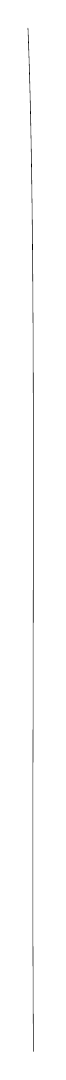
\begin{tikzpicture}[x=1cm,y=1cm]\draw[very thin] (0,0)..controls (.12,-3) and (.04,-9)..(.07,-13);\end{tikzpicture}}}
Or $\overline U$ est fortement 1-acyclique pour $\mathbb L$, donc $H^1(\overline U,\overline g^*\overline F)=0$ et $H^0(\overline U,\overline g^*\overline F)\simeq H^0(\widetilde S,\widetilde F)$. Par suite on a des isomorphismes (``suite spectrale de Hochschild-sSerre en bas dimensions'')
\[
H^1(G,H^0(\widetilde S,\widetilde F))\simeq H^1(\widetilde U,\widetilde g^*\widetilde F)\simeq((R^1j_*)g^*F)_{\overline x},
\]
où $G=\varprojlim_n\mathbb Z/n\mathbb Z=\deleted{\unsure{G(\overline U/U)\ G(\widetilde U/U)}}\ G(\overline U/\widetilde U)$. Puisque $H^0(\widetilde S,\widetilde F)$ \deleted{commutent} et $G$ commutent trivialement au changement de base $\overline s\longrightarrow S$, il en est de même de $(R^1j_*)g^*F$.

Supposons enfin que $F$ soit un faisceau de \deleted{\unsure{$\mathbb L$}} $\mathbb L$-torsion. On va démontrer le théorème sous la forme
\diagram{\[
\begin{tikzcd}
{u'}^*(R^qi^!)g^*F\arrow[r,"\sim"]&(R^q{i'}^!){g'}^*u^*F
\end{tikzcd}
\]}
pour chaque $q$. Puisque le résultat est déjà démontrée pour $q=2$, il est évident de l'argument de recurrence dans la démonstration de (3.7) \deleted{\unsure{qui}} qu'il est \deleted{déjà} également vrai pour $q$ arbitraire dans le cas $F=\mathbb Z/n$ ($n$ premier aux caractéristiques résiduelles). Tenant compte de (VIII.5.5), on termine avec le lemme suivant:
